\documentclass[
11pt, % The default document font size, options: 10pt, 11pt, 12pt
%codirector, % Uncomment to add a codirector to the title page
]{charter} 




% El títulos de la memoria, se usa en la carátula y se puede usar el cualquier lugar del documento con el comando \ttitle
\titulo{Evaluador de microcontroladores para misiones espaciales} 

% Nombre del posgrado, se usa en la carátula y se puede usar el cualquier lugar del documento con el comando \degreename
%\posgrado{Carrera de Especialización en Sistemas Embebidos} 
%\posgrado{Carrera de Especialización en Internet de las Cosas} 
%\posgrado{Carrera de Especialización en Intelegencia Artificial}
%\posgrado{Maestría en Sistemas Embebidos} 
\posgrado{Maestría en Internet de las cosas}

% Tu nombre, se puede usar el cualquier lugar del documento con el comando \authorname
\autor{Gonzalo Nahuel Vaca} 

% El nombre del director y co-director, se puede usar el cualquier lugar del documento con el comando \supname y \cosupname y \pertesupname y \pertecosupname
\director{Roberto Cibils}
\pertenenciaDirector{INVAP} 
% FIXME:NO IMPLEMENTADO EL CODIRECTOR ni su pertenencia
\codirector{Damián Rosetani} % para que aparezca en la portada se debe descomentar la opción codirector en el documentclass
\pertenenciaCoDirector{FIUBA}

% Nombre del cliente, quien va a aprobar los resultados del proyecto, se puede usar con el comando \clientename y \empclientename
\cliente{Roberto Cibils}
\empresaCliente{INVAP}

% Nombre y pertenencia de los jurados, se pueden usar el cualquier lugar del documento con el comando \jurunoname, \jurdosname y \jurtresname y \perteunoname, \pertedosname y \pertetresname.
\juradoUno{Nombre y Apellido (1)}
\pertenenciaJurUno{pertenencia (1)} 
\juradoDos{Nombre y Apellido (2)}
\pertenenciaJurDos{pertenencia (2)}
\juradoTres{Nombre y Apellido (3)}
\pertenenciaJurTres{pertenencia (3)}
 
\fechaINICIO{24 de junio de 2021}		%Fecha de inicio de la cursada de GdP \fechaInicioName
\fechaFINALPlan{19 de agosto de 2021} 	%Fecha de final de cursada de GdP
\fechaFINALTrabajo{15 de mayo de 2022}	%Fecha de defensa pública del trabajo final


\begin{document}

\maketitle
\thispagestyle{empty}
\pagebreak


\thispagestyle{empty}
{\setlength{\parskip}{0pt}
\tableofcontents{}
}
\pagebreak


\section*{Registros de cambios}
\label{sec:registro}


\begin{table}[ht]
\label{tab:registro}
\centering
\begin{tabularx}{\linewidth}{@{}|c|X|c|@{}}
\hline
\rowcolor[HTML]{C0C0C0} 
Revisión & \multicolumn{1}{c|}{\cellcolor[HTML]{C0C0C0}Detalles de los cambios realizados} & Fecha      \\ \hline
0      & Creación del documento                                 &\fechaInicioName \\ \hline
1      & Se completa hasta el punto 6 inclusive                 & 04/07/2021 \\ \hline
2      & Se cambia el nombre del proyecto \newline
		 Se conforma con las políticas de confidencialidad de INVAP \newline
		 Correcciones de redacción \newline
		 Se realiza hasta el punto 8 inclusive                  & 11/07/2021 \\ \hline
3      & Se cambia el logo de FIUBA \newline
         Se actualiza el costo del proyecto \newline
         Se completa hasta el punto 9 inclusive                & 13/07/2021 \\ \hline
%4      & Se completa el plan	                                 & dd/mm/aaaa \\ \hline
\end{tabularx}
\end{table}

\pagebreak



\section*{Acta de constitución del proyecto}
\label{sec:acta}

\begin{flushright}
Buenos Aires, \fechaInicioName
\end{flushright}

\vspace{2cm}

Por medio de la presente se acuerda con el Esp. Ing. \authorname\hspace{1px} que su Trabajo Final de la \degreename\hspace{1px} se titulará ``\ttitle'', consistirá esencialmente en la implementación de un firmware de autocomprobación para el microcontrolador seleccionado y un sistema de inyección de soft-errors, y tendrá un presupuesto preliminar estimado de 600 hs de trabajo y \$500, con fecha de inicio \fechaInicioName\hspace{1px} y fecha de presentación pública \fechaFinalName.

Se adjunta a esta acta la planificación inicial.

\vfill

% Esta parte se construye sola con la información que hayan cargado en el preámbulo del documento y no debe modificarla
\begin{table}[ht]
\centering
\begin{tabular}{ccc}
\begin{tabular}[c]{@{}c@{}}Ariel Lutenberg \\ Director posgrado FIUBA\end{tabular} & \hspace{2cm} & \begin{tabular}[c]{@{}c@{}}\clientename \\ \empclientename \end{tabular} \vspace{2.5cm} \\ 
\multicolumn{3}{c}{\begin{tabular}[c]{@{}c@{}} \supname \\ Director del Trabajo Final\end{tabular}} \vspace{2.5cm} \\
%\begin{tabular}[c]{@{}c@{}}\jurunoname \\ Jurado del Trabajo Final\end{tabular}     &  & \begin{tabular}[c]{@{}c@{}}\jurdosname\\ Jurado del Trabajo Final\end{tabular}  \vspace{2.5cm}  \\
%\multicolumn{3}{c}{\begin{tabular}[c]{@{}c@{}} \jurtresname\\ Jurado del Trabajo Final\end{tabular}} \vspace{.5cm}                                                                     
\end{tabular}
\end{table}




\section{1. Descripción técnica-conceptual del proyecto a realizar}
\label{sec:descripcion}

Las misiones espaciales someten su electrónica a la radiación cósmica.
Por esta razón, se necesitan componentes especiales que fueron sometidos a un largo y costoso proceso de diseño y calificación.
Luego, la tecnología utilizada tiene un elevado costo y retraso tecnológico por sobre los productos del mercado masivo.

Actualmente existe una iniciativa comercial para el empleo en misiones espaciales de componentes sin calificación para uso espacial.
Esta iniciativa es conocida como \emph{New Space} y provee un contexto para el proyecto a realizar.

INVAP necesita evaluar si un microcontrolador en particular puede ser usado en sus misiones espaciales.
El objetivo del proyecto es crear los instrumentos necesarios para realizar la evaluación.
Las herramientas a desarrollar son:

\begin{itemize}
	\item Inyector por consola de comando (CCI)
	\item Proceso de dispositivo bajo prueba (DUT)
\end{itemize}

La radiación cósmica está compuesta por partículas enérgicamente cargadas.
Una de estas partículas puede impactar sobre un microcontrolador.
Si esto ocurre, se produce una \emph{no funcionalidad} debido a un pulso transitorio en la lógica del microcontrolador o sus circuitos de apoyo.
Esta \emph{no funcionalidad} se manifiesta como un \emph{soft-error} no destructivo.
Finalmente, los \emph{soft-errors} son un tipo de error en donde una señal o dato es incorrecto.

Para realizar la inyección de \emph{soft-errors} se propone construir un sistema como se muestra en la figura \ref{fig:diagInyector}.
Se observa que el usuario podrá describir el ensayo a realizar.
Luego, se utilizará un servidor \emph{OCD} para crear las instrucciones del \emph{debugger}.
Finalmente, se inyectarán los errores por protocolo \emph{JTAG}.

\begin{figure}[htpb]
	\centering 
	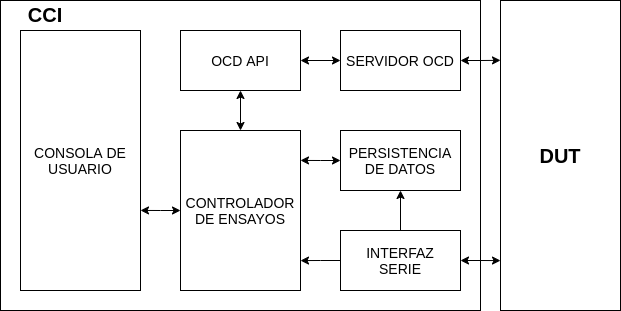
\includegraphics[width=\textwidth]{./Figuras/CCIbloques.png}
	\caption{Diagrama en bloques del Inyector por consola de comando (CCI)}
	\label{fig:diagInyector}
\end{figure}

El segundo módulo del proyecto es el firmware de autocomprobación.
En la figura \ref{fig:diagSelfTesting} se puede observar el diagrama en bloques propuesto.
Como se puede ver, este recurso deberá: verificar el estado de los periféricos, construir un informe y enviar los reportes para su análisis.

\begin{figure}[htpb]
	\centering 
	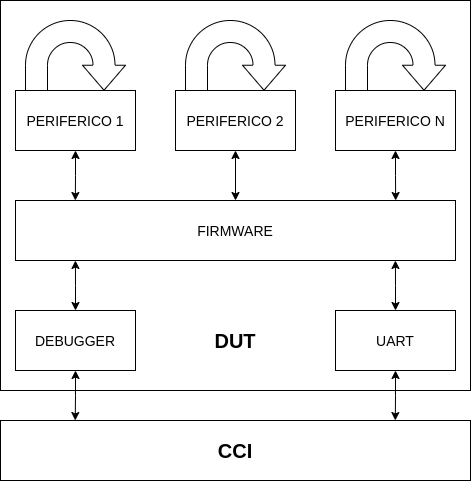
\includegraphics[width=0.8\textwidth]{./Figuras/DUTbloques.png}
	\caption{Diagrama en bloques del Proceso de dispositivo bajo prueba (DUT)}
	\label{fig:diagSelfTesting}
\end{figure}

Se espera que el proyecto agregue valor al INVAP de las siguientes maneras:

\begin{itemize}
	\item Simulando de forma acelerada la duración de una misión espacial
	\item Permitiendo presupuestar nuevo hardware para las misiones futuras
\end{itemize}

\section{2. Identificación y análisis de los interesados}
\label{sec:interesados}

\begin{table}[ht]
%\caption{Identificación de los interesados}
%\label{tab:interesados}
\begin{tabularx}{\linewidth}{@{}|l|X|X|l|@{}}
\hline
\rowcolor[HTML]{C0C0C0} 
Rol           & Nombre y Apellido & Organización 	& Puesto 	\\ \hline
Cliente       & \clientename      &\empclientename	& Ingeniero \\ \hline
Responsable   & \authorname       & FIUBA        	& Alumno 	\\ \hline
Usuario final & Desarrollo de software &\empclientename	& -       	\\ \hline
\end{tabularx}
\end{table}

\begin{itemize}
	\item Cliente: cumple múltiples roles en el proyecto, valorar el tiempo que invierte.
\end{itemize}

\section{3. Propósito del proyecto}
\label{sec:proposito}

El propósito de este proyecto es proporcionar herramientas para:

\begin{itemize}
	\item Medir el nivel de susceptibilidad del software que se ejecuta en el DUT a los efectos de la radiación
	\item Evaluar el origen de dicha susceptibilidad
	\item Comparar la efectividad de distintas estrategias de mitigación incorporadas al software del DUT para mitigar los efectos de la radiación
	\item Obtener la figura de mérito (FOM) del DUT
	\item Simular los efectos del ambiente espacial en un microcontrolador.
	\item Evaluar si un dispositivo del mercado masivo puede ser utilizado en futuras misiones.
\end{itemize}

\section{4. Alcance del proyecto}
\label{sec:alcance}

El proyecto incluye en su alcance la creación de:
\begin{itemize}
	\item Un sistema de inyección de \emph{soft-errors} controlado por consola de comandos
	\item Un firmware de autocomprobación de periféricos para el microcontrolador seleccionado por INVAP
	\item La ejecución de ensayos de \emph{soft-errors} con la finalidad de validar el proyecto
\end{itemize}

El presente proyecto no incluye:

\begin{itemize}
	\item El diseño de ensayos de \emph{soft-errors}
\end{itemize}


\section{5. Supuestos del proyecto}
\label{sec:supuestos}

Para el desarrollo del presente proyecto se supone que:

\begin{itemize}
	\item Se tendrá acceso irrestricto al microcontrolador propuesto por INVAP antes del día 01/01/2022
\end{itemize}


\section{6. Requerimientos}
\label{sec:requerimientos}

Para comprender los requerimientos del proyecto, se enumeran las siguientes definiciones, acrónimos y abreviaturas:

\begin{enumerate}
	\item Definiciones:
	\begin{itemize}
		\item Single event effect: efecto de una partícula enérgicamente cargada sobre un microcontrolador.
		\item Single event funtional interrupt: interrupción causada por el impacto de una sola partícula que conduce a una no funcionalidad temporal.
		\item Single event upset: pulso transitorio en la lógica o circuitos de apoyo. Son \emph{soft-errors} no destructivos.
		\item Soft-error: tipo de error en donde una señal o dato es incorrecto.
	\end{itemize}
	\item Acrónimos:
	\begin{itemize}
		\item API: interfaz de programación de aplicaciones.
		\item DUT: dispositivo bajo prueba (microcontrolador).
		\item FOM: figura de mérito.
		\item IEEE: Instituto de Ingenieros Eléctricos y Electrónicos.
		\item OCD: on-chip debugger.
		\item SEE: single event effect.
		\item SEFI: single event functional interrupt.
		\item SEU: single event upset.
		\item TBD: a ser determinado.
		\item UART: universal asynchronous receiver-trasmitter.
	\end{itemize}
	\item Abreviaturas:
	\begin{itemize}
		\item Std: estándar.
	\end{itemize}
\end{enumerate}

A continuación se enumeran los requerimientos del proyecto según lo especificado en el estándar IEEE Std. 830-1998:

\subsection{Interfaces externas}
\label{sub:interfacesExternas}

\begin{enumerate}
	\item CCI:
	\begin{enumerate}
		\item Con usuario:
		\begin{itemize}
			\item Deberá representar todos los caracteres de ISO Std. 10646
			\item Conformará con las secuencias de escape de ISO Std. 6429
			\item Usará el castellano como idioma conforme a la Real Academia Española
			\item Se aceptarán barbarismos que conformen la interfaz con los sistemas UNIX
			\item No deberá producir destellos ni cambios bruscos en su intensidad lumínica
			\item No deberá producir sonidos
			\item Títulos:
			\begin{itemize}
				\item Los títulos deberán ser cortos
				\item Los títulos deberán estar correctamente capitalizados
				\item Los títulos deberán ser únicos
			\end{itemize}
			\item Comandos:
			\begin{itemize}
				\item El sistema se iniciará con el comando ``python sise.py''
				\item El sistema imprimirá en pantalla un manual de ayuda con el comando ``python sise.py --help''
				\item Se podrá exportar la configuración del último ensayo realizado con el comando ``python sise.py --export=Ruta''
				\item Se podrá importar la configuración de un ensayo a realizar con el comando ``python sise.py --import=Ruta/Archivo''
			\end{itemize}
			\item Menú:
			\begin{itemize}
				\item El sistema de menú tendrá una arquitectura de árbol
				\item La navegación entre los nodos del menú será consistente en todo el árbol
				\item Se indicará en todo momento el nodo actual y todos los nodos que lleven a la raíz del árbol
			\end{itemize}
		\end{itemize}
		\item Con DUT:
		\begin{itemize}
			\item La comunicación con UART será en 9600 baudios, 8 bits de datos, 1 bit de parada y 0 bits de paridad
			\item La comunicación con el debugger conformará con la configuración recomendada por el fabricante
		\end{itemize}
	\end{enumerate}
	\item Proceso de DUT:
	\begin{itemize}
		\item La comunicación con el debugger estará disponible durante todo el flujo de la secuencia
		\item Durante el flujo de la secuencia, la UART solo podrá transmitir información
		\item En el periodo entre secuencias, la UART podrá recibir y transmitir información
	\end{itemize}
\end{enumerate}

\subsection{Funciones}
\label{sub:funciones}

\begin{enumerate}
	\item CCI:
	\begin{itemize}
		\item Detendrá la secuencia de duración $ T $ del DUT en un momento $ t $ definido como \\ $ t \, \epsilon \, \rm I\!R^+ \wedge t \, < T$
		\item Con la secuencia del DUT detenida, inyectará un SEFI-SEU que invertirá el valor de un bit de un registro interno
		\item La descripción del ensayo definirá el momento $ t $ de inyección de SEFI-SEU durante la secuencia de duración $ T $ y será un múltiplo de $\Delta t$ definido como $ \Delta t=T/N \, \forall \, N \epsilon \, \rm I\!N $
		\item La descripción del ensayo definirá la cantidad $ M $ de registros involucrados en la prueba
		\item La cantidad de secuencias $ L $ a ejecutar quedará definida como $ L = N \times M $
		\item Se ejecutará una secuencia de control sin inyección de SEFI-SEU antes de correr las $ L $ secuencias
		\item Por cada ejecución de una secuencia se obtendrá un valor de salida $ S $ del DUT
		\item Cada valor de salida $ S $ será persistido para su análisis
		\item Cada valor de salida $ S $ quedará asociado a su correspondiente secuencia con su inyección de SEFI-SEU y momento $ t $
		\item Se generará un archivo de resultados llamado\\ ``resultados-AAAAMMDDHHmm.res'', siendo AAAA el año del ensayo, MM el mes, DD el día, HH la hora y mm los minutos
		\item El archivo de resultados acumulará los SEFI y SEU de cada registro del DUT
		\item El archivo de resultados acumulará los SEU de cada periférico del DUT
		\item El archivo de resultados indicará el FOM del registro definido como: \\
		$ FOM_{REG} = (1 - \frac{SEU}{SEFI}) $
		\item El archivo de resultados indicará el FOM del DUT definido como: \\
		$ FOM_{DUT} = \frac{1}{M} \times \sum_{i = 1}^{i = M}FOM_{i} $ siendo $ i $ el número que representa un registro del DUT
		\item Se generará un archivo de histogramas llamado ``histogramas-AAAAMMDDmm.his'' siendo AAAA el año del ensayo, MM el mes, DD el día, HH la hora y mm los minutos
		\item El archivo de histogramas tendrá una tabla que indique la frecuencia de fallos como función de los SEFIs por registro del DUT
		\item El archivo de histogramas tendrá una tabla que indique la frecuencia de fallos como función de los SEFIs por periférico del DUT
	\end{itemize}
	\item Proceso de DUT:
	\begin{itemize}
		\item Deberá correr una secuencia de autoevaluación cuya ejecución durará un tiempo $ T $
		\item Deberá producir una salida $ S $ que podrá ser un estado o una secuencia de estados
		\item Este proceso podrá tener una entrada $ E $
		\item Deberá evaluar el estado de los periféricos del DUT
		\item Tendrá una función de evaluación para cada uno de los periféricos del DUT
		\item Se podrá definir por la entrada $ E $ si se desea excluir uno o más periféricos en la secuencia
		\item Manejará una interrupción del flujo normal de la secuencia y generará una salida $ S $ indicando la excepción, por ejemplo: interrupción por \emph{watchdog}
		\item La salida $ S $ utilizará la UART del DUT para ser transmitida
		\item La entrada $ E $ utilizará la UART del DUT para ser recibida
	\end{itemize}
\end{enumerate}

\subsection{Requisitos de rendimiento}
\label{sub:rendimiento}

\begin{itemize}
	\item La inyección de SEFI-SEU podrá tener un desvío en su momento $ t $ de 10 ms
	\item El desvío tolerado de $ t $ deberá representar como máximo el 1\% de la duración $ T $ de la secuencia del DUT
	\item Aceptará un $ \Delta t $ que como mínimo represente el 5\% de la duración $ T $ de la secuencia del DUT
\end{itemize}

\subsection{Restricciones de diseño}
\label{sub:restriccionesDiseño}

\begin{itemize}
	\item Se utilizará como dispositivo principal el microcontrolador seleccionado por INVAP
	\item Se utilizará un sistema operativo de tiempo real para diseñar el Proceso de DUT
\end{itemize}

\subsection{Atributos del sistema}
\label{sub:atributos}

\begin{enumerate}
	\item Mantenibilidad:
	\begin{itemize}
		\item El Proceso de DUT se desarrollará con un modelo de capas
	\end{itemize}
\end{enumerate}

Los requerimientos mencionados se detallan en el documento SISE-RS.

\section{7. Historias de usuarios (\textit{Product backlog})}
\label{sec:backlog}

\begin{itemize}
	\item Como \emph{ingeniero de desarrollo} quiero \emph{simular} los años previstos para una misión espacial en un periodo de 24 hs para \emph{evaluar} las técnicas de mitigación de errores empleadas. \emph{Story points: 8}, la historia de usuario requiere introducir \emph{soft-errors} con una frecuencia proporcional al ensayo.
	\item Como \emph{ingeniero de desarrollo} quiero \emph{obtener} la figura de mérito del microcontrolador seleccionado para \emph{decidir} si el dispositivo es adecuado para la misión. \emph{Story points: 34}, la historia de usuario requiere realizar múltiples secuencias de autovalidación con inyecciones de \emph{soft-errors} precisos.
\end{itemize}


\section{8. Entregables principales del proyecto}
\label{sec:entregables}

Los entregables del proyecto son:

\begin{itemize}
	\item Código fuente en el repositorio con control de versiones \emph{Gitlab} de INVAP
	\item Documentación del código con \emph{Doxygen}
	\item Documentación de las actividades semanales
\end{itemize}


\section{9. Desglose del trabajo en tareas}
\label{sec:wbs}

\begin{enumerate}
\item Planificación
	\begin{enumerate}
	\item Investigación de la problemática (10 hs)
	\item Relevamiento de las necesidades del cliente (15 hs)
	\item Exploración de las posibles tecnologías a emplear (20 hs)
	\item Investigación sobre el nivel de acceso posible al microcontrolador (5 hs)
	\item Creación del documento de especificaciones de requerimientos de software (15 hs)
	\item Elección final de las tecnologías e informe de justificación (15 hs)
	\item Confección de un documento de planificación del proyecto (20 hs)
	\item Reunión de control y aceptación de la documentación (1 hs)
	\item Creación del plan de pruebas y validación (20 hs)
	\item Reunión final de la planificación (1 hs)
	\end{enumerate}
\item Logística e infraestructura
	\begin{enumerate}
	\item Establecimiento de un canal cifrado con el departamento de IT de INVAP (2 hs)
	\item Obtención de credenciales para acceder a la infraestructura de INVAP (2 hs)
	\item Obtención de credenciales para acceder al sistema de control de versiones de INVAP (2 hs)
	\item Configuración del entorno de trabajo conforme a los lineamientos de INVAP (3 hs)
	\item Obtención del hardware necesario para la realización del proyecto (10 hs)
	\end{enumerate}
\item Inyector por consola de comando
	\begin{enumerate}
	\item Integración del servidor OCD (10 hs)
	\item Creacion de los archivos de configuración para el servidor OCD (30 hs)
	\item Pruebas de integración servidor OCD-Dispositivo bajo prueba (10 hs)
	\item Pruebas de rendimiento del servidor OCD (10 hs)
	\item Determinación de la media y desvío del error temporal de SEFI-SEU (5 hs)
	\item Creación de API para el servidor OCD (20 hs)
	\item Pruebas de aceptación de API para el servidor OCD (10 hs)
	\item Determinación y comparación de la media y desvío del error temporal de SEFI-SEU (5 hs)
	\item Servicio de interfaz serie para el dispositivo bajo prueba (20 hs)
	\item Pruebas de rendimiento de la interfaz serie (5 hs)
	\item Servicio de persistencia de datos (20 hs)
	\item Pruebas de aceptación del servicio de persistencia de datos (5 hs)
	\item Codificación del controlador de ensayos (40 hs)
	\item Pruebas del controlador de ensayos (10 hs)
	\item Validación manual de los informes generados (10 hs)
	\item Creación de la consola de usuario (15 hs)
	\item Creación de pruebas automáticas para la consola de usuario (10 hs)
	\item Validación de la consola de usuario por parte del cliente (5 hs)
	\end{enumerate}
\item Proceso en DUT
	\begin{enumerate}
		\item Diseño de la estrategia de autovalidación del estado general del DUT (25 hs)
		\item Diseño de la estrategia de la validación del estado de cada periférico (30 hs)
		\item Análisis de los posibles SEFI-SEU que alteren la secuencia de autovalidación general (25 hs)
		\item Diseño de estrategias de manejo de excepciones (25 hs)
		\item Reunión de control y aceptación del diseño (1 hs)
		\item Codificación del firmware (50 hs)
		\item Pruebas de manejo de excepciones (25 hs)
	\end{enumerate}
\item Procesos de cierre
	\begin{enumerate}
		\item Pruebas automáticas de todo el sistema (6 hs)
		\item Obtención de la figura de mérito del microcontrolador evaluado (1 hs)
		\item Creación de la memoria del trabajo terminado (20 hs)
		\item Creación de la presentación para la defensa pública (5 hs)
		\item Creación del video para la defensa pública (5 hs)
		\item Defensa pública (0,5 hs)
		\item Agradecimiento a todos los involucrados (0,5 hs)
	\end{enumerate}
\end{enumerate}

Cantidad total de horas: (600 hs)

\section{10. Diagrama de Activity On Node}
\label{sec:AoN}

\begin{consigna}{red}
Armar el AoN a partir del WBS definido en la etapa anterior. 

%La figura \ref{fig:AoN} fue elaborada con el paquete latex tikz y pueden consultar la siguiente referencia \textit{online}:

%\url{https://www.overleaf.com/learn/latex/LaTeX_Graphics_using_TikZ:_A_Tutorial_for_Beginners_(Part_3)\%E2\%80\%94Creating_Flowcharts}

\end{consigna}

\begin{figure}[htpb]
\centering 
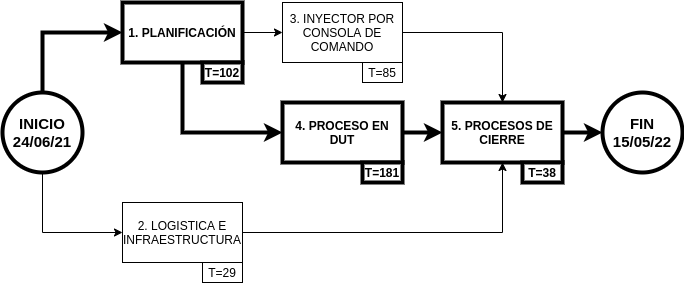
\includegraphics[width=.8\textwidth]{./Figuras/AoN.png}
\caption{Diagrama en \textit{Activity on Node}}
\label{fig:AoN}
\end{figure}

Indicar claramente en qué unidades están expresados los tiempos.
De ser necesario indicar los caminos semicríticos y analizar sus tiempos mediante un cuadro.
Es recomendable usar colores y un cuadro indicativo describiendo qué representa cada color, como se muestra en el siguiente ejemplo:



\section{11. Diagrama de Gantt}
\label{sec:gantt}

\begin{consigna}{red}

Existen muchos programas y recursos \textit{online} para hacer diagramas de gantt, entre los cuales destacamos:

\begin{itemize}
\item Planner
\item GanttProject
\item Trello + \textit{plugins}. En el siguiente link hay un tutorial oficial: \\ \url{https://blog.trello.com/es/diagrama-de-gantt-de-un-proyecto}
\item Creately, herramienta online colaborativa. \\\url{https://creately.com/diagram/example/ieb3p3ml/LaTeX}
\item Se puede hacer en latex con el paquete \textit{pgfgantt}\\ \url{http://ctan.dcc.uchile.cl/graphics/pgf/contrib/pgfgantt/pgfgantt.pdf}
\end{itemize}

Pegar acá una captura de pantalla del diagrama de Gantt, cuidando que la letra sea suficientemente grande como para ser legible. 
Si el diagrama queda demasiado ancho, se puede pegar primero la ``tabla'' del Gantt y luego pegar la parte del diagrama de barras del diagrama de Gantt.

Configurar el software para que en la parte de la tabla muestre los códigos del EDT (WBS).\\
Configurar el software para que al lado de cada barra muestre el nombre de cada tarea.\\
Revisar que la fecha de finalización coincida con lo indicado en el Acta Constitutiva.

En la figura \ref{fig:gantt}, se muestra un ejemplo de diagrama de gantt realizado con el paquete de \textit{pgfgantt}. En la plantilla pueden ver el código que lo genera y usarlo de base para construir el propio.

\begin{figure}[htbp]
\begin{center}
\begin{ganttchart}{1}{12}
  \gantttitle{2020}{12} \\
  \gantttitlelist{1,...,12}{1} \\
  \ganttgroup{Group 1}{1}{7} \\
  \ganttbar{Task 1}{1}{2} \\
  \ganttlinkedbar{Task 2}{3}{7} \ganttnewline
  \ganttmilestone{Milestone o hito}{7} \ganttnewline
  \ganttbar{Final Task}{8}{12}
  \ganttlink{elem2}{elem3}
  \ganttlink{elem3}{elem4}
\end{ganttchart}
\end{center}
\caption{Diagrama de gantt de ejemplo}
\label{fig:gantt}
\end{figure}


\begin{landscape}
\begin{figure}[htpb]
\centering 
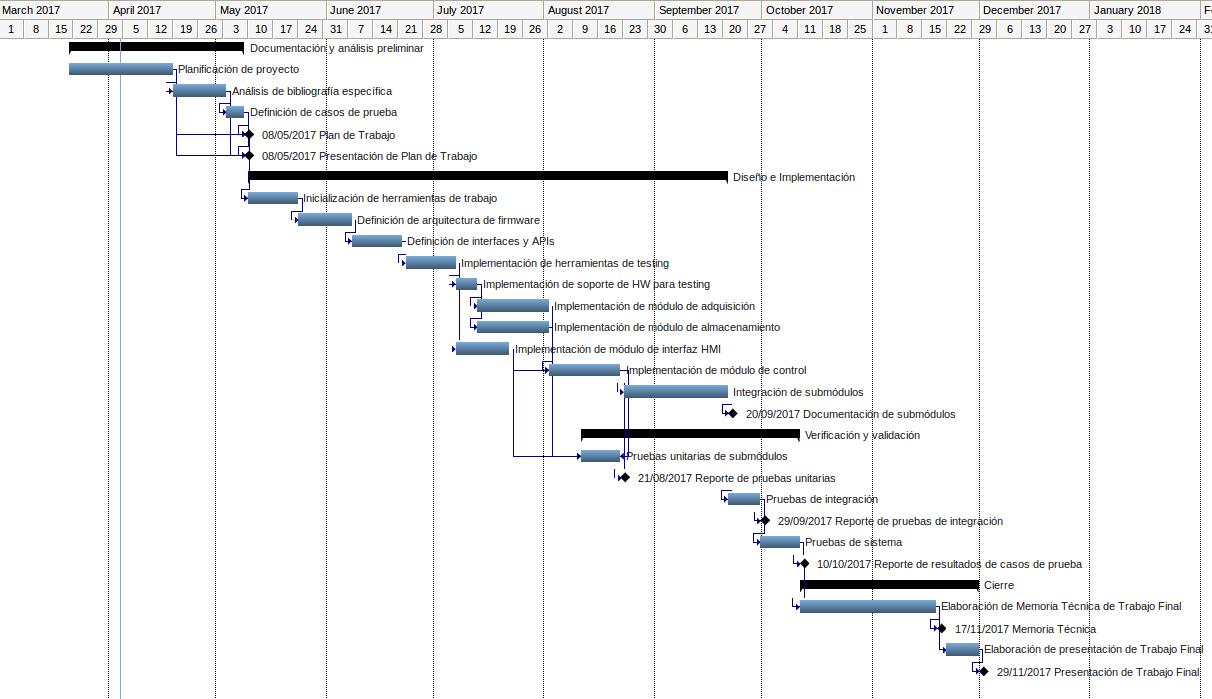
\includegraphics[height=.85\textheight]{./Figuras/Gantt-2.png}
\caption{Ejemplo de diagrama de Gantt rotado}
\label{fig:diagGantt}
\end{figure}

\end{landscape}

\end{consigna}


\section{12. Presupuesto detallado del proyecto}
\label{sec:presupuesto}

\begin{consigna}{red}
Si el proyecto es complejo entonces separarlo en partes:
\begin{itemize}
	\item Un total global, indicando el subtotal acumulado por cada una de las áreas.
	\item El desglose detallado del subtotal de cada una de las áreas.
\end{itemize}

IMPORTANTE: No olvidarse de considerar los COSTOS INDIRECTOS.

\end{consigna}

\begin{table}[htpb]
\centering
\begin{tabularx}{\linewidth}{@{}|X|c|r|r|@{}}
\hline
\rowcolor[HTML]{C0C0C0} 
\multicolumn{4}{|c|}{\cellcolor[HTML]{C0C0C0}COSTOS DIRECTOS} \\ \hline
\rowcolor[HTML]{C0C0C0} 
Descripción &
  \multicolumn{1}{c|}{\cellcolor[HTML]{C0C0C0}Cantidad} &
  \multicolumn{1}{c|}{\cellcolor[HTML]{C0C0C0}Valor unitario} &
  \multicolumn{1}{c|}{\cellcolor[HTML]{C0C0C0}Valor total} \\ \hline
 &
  \multicolumn{1}{c|}{} &
  \multicolumn{1}{c|}{} &
  \multicolumn{1}{c|}{} \\ \hline
 &
  \multicolumn{1}{c|}{} &
  \multicolumn{1}{c|}{} &
  \multicolumn{1}{c|}{} \\ \hline
\multicolumn{1}{|l|}{} &
   &
   &
   \\ \hline
\multicolumn{1}{|l|}{} &
   &
   &
   \\ \hline
\multicolumn{3}{|c|}{SUBTOTAL} &
  \multicolumn{1}{c|}{} \\ \hline
\rowcolor[HTML]{C0C0C0} 
\multicolumn{4}{|c|}{\cellcolor[HTML]{C0C0C0}COSTOS INDIRECTOS} \\ \hline
\rowcolor[HTML]{C0C0C0} 
Descripción &
  \multicolumn{1}{c|}{\cellcolor[HTML]{C0C0C0}Cantidad} &
  \multicolumn{1}{c|}{\cellcolor[HTML]{C0C0C0}Valor unitario} &
  \multicolumn{1}{c|}{\cellcolor[HTML]{C0C0C0}Valor total} \\ \hline
\multicolumn{1}{|l|}{} &
   &
   &
   \\ \hline
\multicolumn{1}{|l|}{} &
   &
   &
   \\ \hline
\multicolumn{1}{|l|}{} &
   &
   &
   \\ \hline
\multicolumn{3}{|c|}{SUBTOTAL} &
  \multicolumn{1}{c|}{} \\ \hline
\rowcolor[HTML]{C0C0C0}
\multicolumn{3}{|c|}{TOTAL} &
   \\ \hline
\end{tabularx}%
\end{table}


\section{13. Gestión de riesgos}
\label{sec:riesgos}

\begin{consigna}{red}
a) Identificación de los riesgos (al menos cinco) y estimación de sus consecuencias:
 
Riesgo 1: detallar el riesgo (riesgo es algo que si ocurre altera los planes previstos de forma negativa)
\begin{itemize}
	\item Severidad (S): mientras más severo, más alto es el número (usar números del 1 al 10).\\
	Justificar el motivo por el cual se asigna determinado número de severidad (S).
	\item Probabilidad de ocurrencia (O): mientras más probable, más alto es el número (usar del 1 al 10).\\
	Justificar el motivo por el cual se asigna determinado número de (O). 
\end{itemize}   

Riesgo 2:
\begin{itemize}
	\item Severidad (S): 
	\item Ocurrencia (O):
\end{itemize}

Riesgo 3:
\begin{itemize}
	\item Severidad (S): 
	\item Ocurrencia (O):
\end{itemize}


b) Tabla de gestión de riesgos:      (El RPN se calcula como RPN=SxO)

\begin{table}[htpb]
\centering
\begin{tabularx}{\linewidth}{@{}|X|c|c|c|c|c|c|@{}}
\hline
\rowcolor[HTML]{C0C0C0} 
Riesgo & S & O & RPN & S* & O* & RPN* \\ \hline
       &   &   &     &    &    &      \\ \hline
       &   &   &     &    &    &      \\ \hline
       &   &   &     &    &    &      \\ \hline
       &   &   &     &    &    &      \\ \hline
       &   &   &     &    &    &      \\ \hline
\end{tabularx}%
\end{table}

Criterio adoptado: 
Se tomarán medidas de mitigación en los riesgos cuyos números de RPN sean mayores a...

Nota: los valores marcados con (*) en la tabla corresponden luego de haber aplicado la mitigación.

c) Plan de mitigación de los riesgos que originalmente excedían el RPN máximo establecido:
 
Riesgo 1: plan de mitigación (si por el RPN fuera necesario elaborar un plan de mitigación).
  Nueva asignación de S y O, con su respectiva justificación:
  - Severidad (S): mientras más severo, más alto es el número (usar números del 1 al 10).
          Justificar el motivo por el cual se asigna determinado número de severidad (S).
  - Probabilidad de ocurrencia (O): mientras más probable, más alto es el número (usar del 1 al 10).
          Justificar el motivo por el cual se asigna determinado número de (O).

Riesgo 2: plan de mitigación (si por el RPN fuera necesario elaborar un plan de mitigación).
 
Riesgo 3: plan de mitigación (si por el RPN fuera necesario elaborar un plan de mitigación).

\end{consigna}


\section{14. Gestión de la calidad}
\label{sec:calidad}

\begin{consigna}{red}
Para cada uno de los requerimientos del proyecto indique:
\begin{itemize} 
\item Req \#1: copiar acá el requerimiento.

\begin{itemize}
	\item Verificación para confirmar si se cumplió con lo requerido antes de mostrar el sistema al cliente. Detallar 
	\item Validación con el cliente para confirmar que está de acuerdo en que se cumplió con lo requerido. Detallar  
\end{itemize}

\end{itemize}

Tener en cuenta que en este contexto se pueden mencionar simulaciones, cálculos, revisión de hojas de datos, consulta con expertos, mediciones, etc.  Las acciones de verificación suelen considerar al entregable como ``caja blanca'', es decir se conoce en profundidad su funcionamiento interno.  En cambio, las acciones de validación suelen considerar al entregable como ``caja negra'', es decir, que no se conocen los detalles de su funcionamiento interno.

\end{consigna}

\section{15. Procesos de cierre}    
\label{sec:cierre}

\begin{consigna}{red}
Establecer las pautas de trabajo para realizar una reunión final de evaluación del proyecto, tal que contemple las siguientes actividades:

\begin{itemize}
	\item Pautas de trabajo que se seguirán para analizar si se respetó el Plan de Proyecto original:
	 - Indicar quién se ocupará de hacer esto y cuál será el procedimiento a aplicar. 
	\item Identificación de las técnicas y procedimientos útiles e inútiles que se emplearon, y los problemas que surgieron y cómo se solucionaron:
	 - Indicar quién se ocupará de hacer esto y cuál será el procedimiento para dejar registro.
	\item Indicar quién organizará el acto de agradecimiento a todos los interesados, y en especial al equipo de trabajo y colaboradores:
	  - Indicar esto y quién financiará los gastos correspondientes.
\end{itemize}

\end{consigna}


\end{document}
